% #📘 Chapter4_ChannelEstimationEqualization.tex

\chapter{Channel Estimation and Equalization}

\section{Introduction}
In a wireless communication system, signals propagate through a channel that introduces distortion due to multipath fading, noise, and Doppler shifts. To reliably decode the transmitted data, the receiver must estimate the channel and apply equalization techniques to mitigate these effects.

\section{Channel Effects}

\subsection{Multipath Fading}
A transmitted signal reaches the receiver through multiple paths, causing constructive and destructive interference.

\begin{itemize}
  \item Delay spread leads to Inter-Symbol Interference (ISI)
  \item Coherence bandwidth determines frequency selectivity
\end{itemize}

\subsection{Noise and Doppler Effects}
The wireless channel also adds additive white Gaussian noise (AWGN) and may cause Doppler shift due to user mobility.

\section{Channel Models}

\subsection{Flat Fading vs. Frequency Selective Fading}
\begin{itemize}
  \item Flat fading: Channel gain is constant across bandwidth
  \item Frequency selective fading: Channel varies across subcarriers
\end{itemize}

\subsection{Mathematical Model}
For a baseband channel:
\[
r(t) = h(t) * s(t) + n(t)
\]
Where:
\begin{itemize}
  \item $r(t)$ is the received signal
  \item $h(t)$ is the channel impulse response
  \item $s(t)$ is the transmitted signal
  \item $n(t)$ is additive noise
\end{itemize}

\section{Channel Estimation Techniques}

\subsection{Pilot-Based Estimation}
Transmit known pilot symbols at predefined locations. Estimate channel response based on received pilot values.

\[
\hat{h} = \frac{y_p}{x_p}
\]

\subsection{Least Squares (LS) Estimation}
Minimizes the squared error between received and estimated values.

\[
\hat{h}_{LS} = (X^H X)^{-1} X^H y
\]

\subsection{Minimum Mean Squared Error (MMSE) Estimation}
Takes noise and channel statistics into account.

\[
\hat{h}_{MMSE} = R_{hy} R_{yy}^{-1} y
\]

\section{Equalization Techniques}

\subsection{Zero Forcing Equalizer (ZF)}
Inverts the channel matrix assuming no noise.

\[
\hat{x} = (H^H H)^{-1} H^H y
\]

\subsection{MMSE Equalizer}
Balances inversion and noise suppression.

\[
\hat{x}_{MMSE} = (H^H H + \sigma^2 I)^{-1} H^H y
\]

\section{OFDM Channel Estimation}
OFDM uses pilot subcarriers across time and frequency.

\begin{figure}[H]
    \centering
    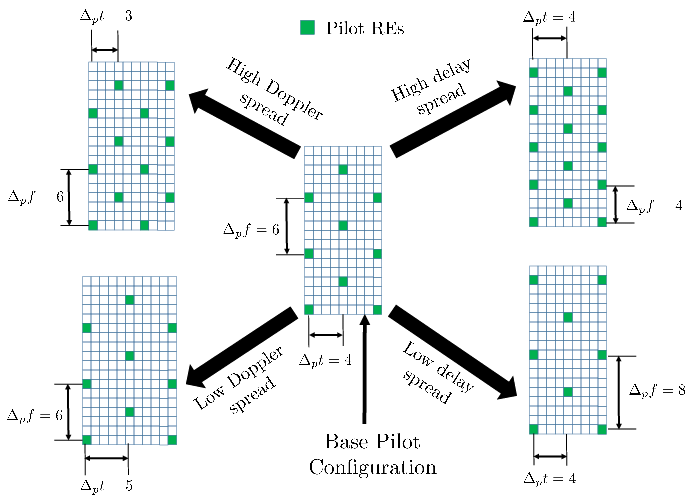
\includegraphics[width=0.7\textwidth]{images/ofdm_pilot_grid.png}
    \caption{Pilot placement in time-frequency grid of OFDM.}
\end{figure}

\section{Conclusion}
Accurate channel estimation and equalization are crucial for reliable communication in fading environments. In modern systems like 5G, advanced equalizers are paired with MIMO and OFDM to enhance performance.

\section*{Further Reading}
\begin{itemize}
  \item Rappaport, T. S. (2010). \textit{Wireless Communications: Principles and Practice}.
  \item Tse, D., \& Viswanath, P. (2005). \textit{Fundamentals of Wireless Communication}.
\end{itemize}

